% Elsevier Journal Paper Template
% Using elsarticle document class with review mode
\documentclass[final,3p,times,review,sort&compress]{elsarticle}


% === Required Packages ===
\usepackage[utf8]{inputenc}
\usepackage[T1]{fontenc}
\usepackage{amsmath,amssymb,amsfonts}
\usepackage{lineno}
\linenumbers
\usepackage{graphicx}
\usepackage{booktabs}          % Professional tables (\toprule, \midrule, \bottomrule)
\usepackage{tabularx}          % Full-width tables
% cite package not needed: elsarticle loads natbib internally
\usepackage[ruled,linesnumbered]{algorithm2e}  % Algorithm environment
\usepackage{xcolor}            % Colors
\usepackage{url}               % URL formatting
\usepackage{xspace}            % Smart spacing for macros
\usepackage{pifont}            % Dingbats (\ding{51} checkmark, \ding{55} cross)
% amsthm not loaded: elsarticle provides its own theorem environments
\newdefinition{proposition}{Proposition}

% === Optional Packages ===
% \usepackage{subfig}          % Subfigures (IEEE preferred over subcaption)
% \usepackage{multirow}        % Multi-row table cells
% \usepackage{balance}         % Balance columns on last page

% === Hyperref (load last, optional for camera-ready) ===
\usepackage{hyperref}
\hypersetup{
    colorlinks=true,
    linkcolor=red,
    citecolor=red,
    urlcolor=red,
    pdfauthor={Author A, Author B, Author C},
    pdftitle={Cross-Layer Coordination for Fresh and Reliable Data Acquisition in Smart Transportation Systems}
}

% === Custom Commands ===
\newcommand{\eg}{e.g.,\xspace}
\newcommand{\ie}{i.e.,\xspace}
\newcommand{\etal}{et~al.\xspace}
\newcommand{\wrt}{w.r.t.\xspace}
\newcommand{\cf}{cf.\xspace}

% === Paper Metadata ===
\journal{Alexandria Engineering Journal}

\title{Cross-Layer Coordination for Fresh and Reliable Data Acquisition in Smart Transportation Systems}

\author[inst1]{Shasha Xia}
\ead{xia.shasha@outlook.com}
\author[inst2]{Baohui Zhang}
\ead{y125211005@stu.ahu.edu.cn}
\author[inst2]{Jianwei Tai\corref{cor1}}
\ead{taijianwei1993@163.com}

\cortext[cor1]{Corresponding author. taijianwei1993@163.com}
\affiliation[inst1]{organization={Institute of Dataspace, Hefei Comprehensive National Science Center, 230088. 
},
  city={Hefei},
  country={China}}
\affiliation[inst2]{organization={School of Internet, Anhui University, 230601 },
  city={Hefei},
  country={China}}

% Method Name: CoTDA
\begin{document}

\begin{frontmatter}

% === Abstract ===
\begin{abstract}
High-fidelity perception in smart transportation systems requires the timely delivery of massive sensor data to fusion centers, yet the freshness of this information is often degraded by uncoordinated cross-layer latencies. Existing V2X architectures typically optimize sensing selection, compression, and multi-hop forwarding in isolation, failing to account for the performance trade-offs inherent in the end-to-end pipeline. This paper introduces \textbf{CoTDA}, a cross-layer coordination framework that treats the sensing-to-delivery chain as a single, constrained optimization problem. CoTDA jointly executes three critical per-slot decisions: urgency-aware admission gating, adaptive discrete compression, and reliability-weighted multi-hop routing. We formulate this joint problem as an NP-hard multi-commodity flow problem with binary source activation and solve it via a three-stage sequential decomposition integrated with a Proximal Policy Optimization (PPO) policy. A lightweight delivery-reliability feedback loop closes the control cycle, providing practical resilience against unreliable agents without the computational overhead of blockchain-based consensus. Evaluated on SUMO-simulated V2X environments and real-world trajectories from the pNEUMA dataset, CoTDA reduces the weighted Age of Information (AoI) by 22--30\% and improves data utility by 17--23\% over state-of-the-art partial baselines. Furthermore, our resilience analysis demonstrates that while the feedback mechanism maintains utility within 8\% of the baseline under random-noise adversaries, it identifies the operational bounds of the architecture under adaptive colluding attacks. The system maintains a sub-40\,ms computational latency, confirming its suitability for real-time vehicular deployment.
\end{abstract}

% === Keywords ===
\begin{keyword}
Age of Information \sep cross-layer coordination \sep vehicular edge computing \sep multi-hop routing \sep data compression \sep V2X communication
\end{keyword}

\end{frontmatter}

\section{Introduction}
\label{sec:introduction}

Modern smart transportation systems rely on dense networks of roadside units (RSUs), connected vehicles, and multi-modal sensors that continuously produce perception data for collision avoidance, signal-free intersection management, and cooperative platooning. The volume and velocity of this data are growing rapidly, driven by edge-accelerated detectors like GC-YOLOv9 that process hundreds of frames per second at the network's periphery. Yet, the raw detections must traverse heterogeneous 5G and IoT fabrics before traffic planners and autonomous controllers can act on them~\cite{AN2024277}. A systematic mapping of 5G-enabled smart-city deployments confirms that transportation is the most data-intensive application domain, imposing latency, reliability, and spectrum-orchestration requirements that existing network stacks satisfy only partially~\cite{YANG2022200065}. As sensor coverage expands, the end-to-end pipeline between perception and actuation emerges as the primary performance bottleneck: in a high-speed autonomy loop, a stale detection is often more dangerous than a missing one, as it targets an incorrect spatial-temporal state. The critical limiting factor is thus no longer sensing range or processing speed alone, but rather the cross-layer orchestration required to deliver sensed information while it remains actionable for downstream control.

Three intertwined technical challenges prevent this perception-to-actuation pipeline from scaling effectively. First, the freshness of transmitted data, formally measured by the Age of Information (AoI) metric, is highly sensitive to the multi-hop queuing and forwarding delays inherent in vehicular networks. Mohammed~et~al.~\cite{MOHAMMED2025111706} demonstrate that even age-priority packet management must carefully balance preemption overhead against update frequency to maintain freshness in multi-user V2X scenarios. Second, vehicular links alternate between sub-6\,GHz channels with moderate capacity and millimetre-wave (mmWave) beams that offer high throughput but suffer frequent, unpredictable blockage due to mobility and obstacles~\cite{HE2023100610}. Third, as sensing becomes a collaborative effort across public RSUs and private fleets, data provenance becomes a first-class concern. While blockchain-backed V2X architectures can authenticate sources, their consensus latencies and energy costs frequently conflict with the stringent freshness goals of the control loop~\cite{SARKAR2022100533}. Solving these challenges in isolation leads to sub-optimal system performance: a perfect AoI scheduler may waste bandwidth on unreliable sources, while a high-throughput mmWave link may be ineffectively shared if the sensing gating logic is overly conservative. This fundamental coupling demands a cross-layer design that treats sensing admission, data compression, and multi-hop forwarding as a unified optimization target.

Several recent systems address individual segments of this pipeline, yet they typically treat the upstream data-selection and downstream network-transport as isolated stages. Jeon and Jeong~\cite{JEON20123318} apply partially observable Markov decision processes (POMDP) to adaptive sensing in cognitive radio networks, focusing on when to sense primary-user bands, yet the framework stops at the physical layer and does not propagate admission decisions through a multi-hop fabric. At the network plane, Kang~et~al.~\cite{KANG2026111852} proposed a Lyapunov-guided reinforcement learning (DRL) controller for RSU offloading that optimizes queue stability; however, their model assumes that all perception features are static workloads, ignoring the possibility of adjusting compression or gating at the source. More coordinated intersection-level approaches like T3C~\cite{WU2024104886} jointly optimize vehicle trajectories and communication, but their scope remains limited to local geometry and does not scale to city-wide multi-hop routing. Similarly, context-aware V2V fog computing~\cite{RAHMAN2020100236} and transfer-learning-based offloaders like TMx-TORU~\cite{AKYILDIZ2026108292} significantly reduce task-failure rates and latency, but because they decouple sensing priorities from routing participation, the upstream data-gating stage and the downstream delivery stage remain independently optimized. This decoupling leads to a "decomposition loss" where sensing agents produce data that cannot be routed, or high-capacity routes carry stale information that provides little utility to the consumer.

We propose \textbf{CoTDA}, a framework that treats the entire sensing-to-delivery chain as a single per-slot constrained optimization problem. A freshness-aware utility function simultaneously determines which agents are admitted into the network, at what discrete compression level, and along which multi-hop path, subject to time-varying link capacities and per-agent reliability budgets. At each scheduling interval, the admission module evaluates every sensing agent through a gating score that combines an urgency signal—derived from the agent's current AoI—with a learned content-relevance term representing its historical contribution to the fusion task. Compression levels are selected from a discrete candidate set following the resource-allocation philosophy of~\cite{SEKARAN2021107649}, allowing the scheduler to balance distortion against the dual costs of bandwidth and energy. The multi-hop planner assigns paths via Lagrangian relaxation, with dual-variable warm-starts across slots to minimize computational overhead in highly dynamic topologies~\cite{AKYILDIZ2026108292}. A lightweight delivery-reliability feedback loop adjusts agent scores so that unreliable sources triggering retransmissions are penalized in future rounds, ensuring system-level accountability without the heavy consensus costs of traditional blockchain frameworks~\cite{SARKAR2022100533}.

From a theoretical perspective, the coordination in CoTDA addresses the optimality gap inherent in modular vehicular stacks. In a modular design, the sensing stage identifies "important" data without knowledge of current multi-hop congestion, while the routing stage treats all incoming packets as high-priority workloads. This lack of transparency forces the system to over-provision either the sensing rate or the link capacity, leading to the "bufferbloat" phenomenon where high-throughput links Paradoxically increase end-to-end AoI due to oversized queues. In contrast, CoTDA’s per-slot coordination enables a "broad-coverage, graded-fidelity" strategy: it prioritizes admitting stale agents at high compression to provide a low-fidelity refresh across the entire network (reducing global AoI), while allocating high-fidelity slots only to those agents with critical content relevance and available high-throughput routing. By redistributing resources across admission, compression, and routing layers in real-time, CoTDA achieves a fresh and reliable data acquisition state that independently tuned modules cannot reach.

The main contributions of this paper are organized as follows:
\begin{itemize}
    \item We propose a cross-layer coordination framework, \textbf{CoTDA} (Section~\ref{sec:method}), that jointly optimizes sensing gating, discrete compression, and multi-hop routing via a per-slot Lagrangian relaxation with PPO-integrated dual warm-starts.
    \item We introduce a delivery-reliability feedback mechanism (Section~\ref{subsec:trust_robust}) that uses semantic consistency and delivery outcomes to dynamically update agent admission scores, providing a lightweight alternative to blockchain-based trust management.
    \item We conduct an extensive evaluation (Section~\ref{sec:experiments}) using SUMO-simulated V2X environments and real-world trajectories from the pNEUMA dataset. Results demonstrate that CoTDA reduces the weighted Age of Information (AoI) by 22--30\% while maintaining a sub-40\,ms per-slot computational latency.
\end{itemize}
The remainder of this paper is organized as follows. Section~\ref{sec:related} reviews related work, Section~\ref{sec:method} details the CoTDA architecture, Section~\ref{sec:experiments} presents the experimental results, and Section~\ref{sec:conclusion} summarizes our findings and future directions.

% === Related Work ===
\section{Related Work}
\label{sec:related}

\subsection{Freshness-aware sensing and transmission}
Keeping traffic observations timely from the moment a sensor captures them to the moment a controller consumes them is a long-standing problem.  Edge-accelerated detection pipelines such as GC-YOLOv9 push annotated frames from cameras to city-level dashboards within milliseconds, yet they treat downstream scheduling and transport as an opaque pipe whose delay is tolerable rather than controllable~\cite{AN2024277}.  Complementary work on the Age of Information (AoI) metric shifts attention to the receiving end: the AP-LGFS strategy, for example, dynamically preempts ongoing transmissions whenever a newly arrived packet exhibits a lower expected AoI, achieving tighter freshness bounds in multi-user V2X channels~\cite{MOHAMMED2025111706}.  Such queuing-layer solutions, however, assume that the sensing rate and data volume upstream are given, ignoring how compression or selective gating at the source could further reduce staleness.

Moving one layer deeper, cross-layer VANET designs argue that routing, MAC, and application concerns must be jointly addressed~\cite{JARUPAN2011966}, and cooperative V2X protection schemes show that coordinated perception messages among heterogeneous road users improve detection recall but compound the bandwidth demand~\cite{HEJAZI2024110396}.  When predictive control enters the picture, whether through physics-enhanced residual learning for oscillation damping~\cite{LONG2024100154} or deep Koopman operators for mixed-traffic stabilization~\cite{LYU2026104258}, the upstream sensing load becomes a function of the controller's prediction horizon, yet no closed-loop mechanism feeds link-quality information back into the sensing schedule.  Federated approaches such as V-FedMM illustrate how sample and vehicle selection can be co-optimized under per-round delay constraints~\cite{TU2026112020}, and POMDP-based cognitive-radio schedulers show how partial observability can guide sensing decisions adaptively~\cite{JEON20123318}.  The traffic-communication coupling framework T3C~\cite{WU2024104886} and dual-band V2X schedulers that account for data importance and freshness decay~\cite{HE2023100610} come closest to bridging sensing and transmission, but both remain scoped to a single intersection or a fixed batch of packets.

In this context, CoTDA generalizes these ideas by closing the loop across all three layers: a sensing gating policy, a compression-fidelity selector, and a multi-hop forwarding scheduler operate under a single objective that minimizes weighted AoI subject to bandwidth and trust budgets, so that upstream data selection directly shapes downstream routing decisions.

\subsection{Multi-hop offloading and resource-aware control}
Vehicular Edge Computing (VEC) and Vehicular Fog Computing (VFC) extend cloud resources to the road, and the dominant research question is \emph{where} and \emph{how much} of a task to offload.  DRL-based controllers have progressed from single-hop schemes, including DDPG schedulers that minimize system cost in MEC environments~\cite{ZHAO2023103193} and fuzzy-RL policies that balance RSU energy with task deadlines along rural highways~\cite{VEMIREDDY2021108463}, to multi-hop architectures that exploit V2V relays.  Ahmed et al.\ formulate multi-hop VEC offloading with PPO-based mobility analysis and 5G\,NR mmWave back-haul~\cite{AHMED2024101854}, while hybrid heuristic relay selection targets energy-optimal hop counts through a multi-objective function of link reliability, outage probability, and transmission delay~\cite{KIRAN2023103058}.  More recent work adds stability awareness: Li et al.\ couple a link-lifetime model with MADDPG to handle the scheduling fragility that vehicle mobility induces~\cite{LI2026103079}, PORA-MATD3 splits each task into partial offloads whose residuals can migrate when a vehicle exits an RSU's range~\cite{XUE2025108081}, and Zhou et al.\ apply a multi-agent Transformer with auto-regressive coordination to NOMA-based VEC, jointly optimizing power control and offloading to maximize service success rate~\cite{ZHOU2026104222}.  A recent VFC offloading survey confirms that the joint effects of latency, energy, and mobility remain insufficiently addressed by any single optimization paradigm~\cite{SNEHA2026110847}.

At the control-plane level, Lyapunov-guided frameworks such as A-F-SCD transform long-horizon R2X objectives into per-slot decisions, combining SAC and DDPG with attention-fused actor networks and prioritised experience replay~\cite{KANG2026111852}.  TMx-TORU further shows that transfer learning across prior offloading routes can cut selection overhead by up to 40\%, though it assumes input features are already generated and thus cannot influence what data is collected~\cite{AKYILDIZ2026108292}.  TD3-based ratio offloading between RSUs and AN-MEC tiers achieves decision times five orders of magnitude faster than simulated annealing~\cite{YAHYA2025100862}, and context-aware V2V fog computing demonstrates that direction- and speed-aware relay selection reduces task-failure rates by up to 10\%~\cite{RAHMAN2020100236}, while proximal on-policy MADRL further decouples mode selection from resource assignment in dense V2X topologies~\cite{BUDHIRAJA2024268}.  Mixed sub-6\,GHz/mmWave scheduling captures heterogeneous link types but maximizes routing utility for fixed data batches, leaving freshness-driven admission control unaddressed~\cite{HE2023100610}.

Unlike these offloading frameworks that treat upstream data as a given workload, CoTDA fuses sensing urgency with spectrum choice and transfer-learning-informed relay selection within a single control loop, so that upstream data gating directly constrains the offloading graph and vice versa.

\subsection{Security-aware resilience and spectrum selection}
Once multi-stakeholder V2X data flows cross organizational boundaries, trust and spectrum management become entangled constraints.  Blockchain-backed vehicular NDN caches reputation scores on-chain to filter forged Interest and Data packets, but the consensus overhead inflates per-hop latency~\cite{KHELIFI2020106715}.  Neural-synchronization-enhanced blockchain provides mutual V2V/V2I authentication and payment, yet its cloud-mediated architecture introduces a centralization bottleneck that conflicts with low-latency goals~\cite{SARKAR2022100533}.  Lighter-weight alternatives exist: BLS-signature-based authentication with reputation revocation achieves sub-8\,ms verification for 5G-V2X messages~\cite{ABDELHAKEEM2023101638}, and the recent cross-layer telematics-security survey confirms that existing defences address intra-vehicle, V2X, and cloud layers in isolation, failing to secure data flows across architectural boundaries~\cite{WU2026101024}.

On the spectrum side, AI-driven allocation has matured from greedy fractional-knapsack/Lagrange-hyperplane frameworks that reduce access delay in 5G IoT sensor networks~\cite{SEKARAN2021107649} to RL-DSA, a hierarchical multi-agent RL controller with digital-twin stress testing and adversarial training that targets next-generation CRN topologies~\cite{VENKATESAN2026112217}.  Reputation-based resource prioritisation (RPRA) in VFC uses subjective-logic trust to evict rogue fog nodes, but its static weight allocation cannot adapt to time-varying freshness requirements~\cite{KHATTAK2024103401}.  Cooperative QoS frameworks that couple firefly-optimized multi-constraint routing with game-theoretic incentive modules and authentication layers illustrate that robustness, cooperation, and security can be co-designed, although they do not account for AoI or data-provenance coupling~\cite{RAJPUT2022100423}.  The systematic mapping of 5G smart-city deployments by Yang~et~al.~\cite{YANG2022200065} reinforces this point: latency, reliability, and spectrum orchestration must be coordinated across heterogeneous IoT/transportation services.

CoTDA distinguishes itself by embedding lightweight provenance checks and market-aware priority scoring into the forwarding path so that trust verification costs are budgeted alongside AoI and bandwidth, rather than being optimized in a separate security layer.

Unlike prior work that treats sensing selection, compression, forwarding, and trust verification as isolated layers, CoTDA is formulated as a single constrained problem. This coordination lets the framework redistribute resources across layers to maximize data freshness within bandwidth and trust budgets.


% === Method ===
\section{Proposed Architecture: CoTDA}
\label{sec:method}

CoTDA formalizes the sensing-to-delivery pipeline as a joint optimization problem across discrete time slots $t\in\{1,\dots,T\}$, addressing the coordination gaps identified in Section~\ref{sec:introduction}. We describe the system model and problem formulation (Section~\ref{subsec:problem}) followed by the framework overview (Section~\ref{subsec:overview}) and the core modules---urgency-aware acquisition, adaptive compression, and reliability-weighted routing---before detailing the closed-loop feedback mechanism and training procedure.

\subsection{System Model and Problem Formulation}
\label{subsec:problem}

We model the sensing-to-delivery pipeline as a sequence of discrete time slots $t\in\{1,\dots,T\}$. Let $\mathcal{V}$ index the set of $V$ sensing agents (vehicles, RSUs, roadside cameras) and $\mathcal{L}$ denote the set of candidate communication links spanning V2V, V2I sub-6\,GHz, and mmWave bands. At each slot $t$, agent $v\in\mathcal{V}$ produces a sensed feature vector $\mathbf{s}_v^t\in\mathbb{R}^{d}$ and is characterized by a compute budget $c_v^t$ and a geographic position $\mathbf{p}_v^t$. Each link $\ell\in\mathcal{L}$ exposes an instantaneous capacity $B_\ell^t$ and a reliability score $r_\ell^t\in[0,1]$ that captures blockage probability, following the dual-band formulation in~\cite{HE2023100610}.

\paragraph{Age of Information}
We adopt AoI as the primary freshness metric. Let $g_v^t$ denote the generation time of agent $v$’s most recently delivered packet at slot $t$. The instantaneous AoI at the fusion center is
\begin{equation}
\Delta_v^t = t - g_v^t,
\label{eq:aoi_def}
\end{equation}
and we derive two complementary scores from it (Eq.~\ref{eq:aoi_def}). The \emph{freshness score} $w_v^t = e^{-\alpha\Delta_v^t}$ ($\alpha>0$) is high when agent $v$'s data is recent and low when it is stale; it acts as a value multiplier in the objective, so that delivering fresh data yields a larger reward. The \emph{urgency score} $u_v^t = 1 - e^{-\alpha\Delta_v^t}$ is the complement: it grows with staleness and drives the admission gate (Section~\ref{subsec:acquisition}) to prioritise agents whose last delivery was long ago. Separating these two quantities avoids conflating ``how valuable a delivery is'' (freshness, used in Eq.~\eqref{eq:objective}) with ``how badly an agent needs to transmit'' (urgency, used in the gating score Eq.~\eqref{eq:qvalue}), consistent with age-priority preemption policies~\cite{MOHAMMED2025111706}.

\paragraph{Decision variables}
The scheduler must jointly determine three quantities per agent per slot: an admission indicator $z_v^t\in\{0,1\}$, a compression ratio $\rho_v^t\in[0,1]$ that reduces the transmitted feature dimension to $d(1-\rho_v^t)$, and a multi-hop forwarding path $\pi_v^t$ through the link overlay.

\paragraph{Objective}
We seek to maximize the time-averaged freshness-weighted utility subject to bandwidth, compute, and provenance constraints:
\begin{equation}
\max_{z,\rho,\pi}\;\frac{1}{T}\sum_{t=1}^{T}\sum_{v\in\mathcal{V}} w_v^t\, z_v^t\, \mathcal{U}_{v\to\pi_v^t} - \lambda_{\rho}\|\boldsymbol{\rho}^t\|_1 - \lambda_{\pi}\sum_{v} \mathcal{C}_{\mathrm{prov}}(\pi_v^t)
\label{eq:objective}
\end{equation}
\begin{align}
\text{s.t.}\quad & \sum_{v:\ell\in\pi_v^t} z_v^t\,(1{-}\rho_v^t)\,d \;\leq\; B_\ell^t, \quad \forall\,\ell\in\mathcal{L},\; \forall\,t, \label{eq:bw_constr}\\
& z_v^t\,c_v^{\mathrm{comp}}(\rho_v^t) \;\leq\; c_v^t, \quad \forall\,v\in\mathcal{V},\; \forall\,t, \label{eq:compute_constr}\\
& \mathcal{C}_{\mathrm{prov}}(\pi_v^t) \;\leq\; \tau_v^t, \quad \forall\,v:\;z_v^t{=}1,\; \forall\,t, \label{eq:trust_constr}
\end{align}
where $\mathcal{U}_{v\to\pi}$ aggregates reliability, capacity, and spectrum cost along path $\pi$ (defined in Eq.~\ref{eq:path_util}), $c_v^{\mathrm{comp}}(\rho_v^t)$ is the compression compute cost, $\mathcal{C}_{\mathrm{prov}}(\pi)$ accumulates per-hop provenance consumption, and $\tau_v^t$ is agent $v$’s rolling trust budget (Section~\ref{subsec:provenance}). The $\lambda$ terms regularize compression aggressiveness and path trustworthiness. Constraint~\eqref{eq:bw_constr} enforces per-link bandwidth limits (analogous to scheduling constraints in~\cite{HE2023100610}); constraint~\eqref{eq:compute_constr} caps per-agent compression cost; and constraint~\eqref{eq:trust_constr} prevents routing through paths whose cumulative provenance exceeds the agent’s earned trust.

Problem \eqref{eq:objective}--\eqref{eq:trust_constr} is NP-hard: even with fixed $\rho$ and $\tau$, the binary admission and multi-commodity routing variables reduce to a capacitated multi-commodity flow problem with binary source activation~\cite{KIRAN2023103058}. We decompose the problem into three tractable stages---acquisition, compression, and routing---treating each decision variable class sequentially as described in the following subsections. Table~\ref{tab:notation} summarizes the notation.

\begin{table}[t]
\centering
\caption{Key notation for CoTDA.}
\label{tab:notation}
\begin{tabularx}{\columnwidth}{lX}
\toprule
\textbf{Symbol} & \textbf{Description} \\
\midrule
$\mathcal{V},\;\mathcal{L}$ & Set of sensing agents; set of candidate links/bands \\
$\mathbf{s}_v^t\in\mathbb{R}^d$ & Raw feature vector produced by agent $v$ at slot $t$ \\
$\Delta_v^t$ & Instantaneous AoI of agent $v$ \\
$w_v^t,\;u_v^t$ & Freshness score ($e^{-\alpha\Delta}$) and urgency score ($1-e^{-\alpha\Delta}$) \\
$z_v^t\in\{0,1\}$ & Admission indicator (1 = agent transmits) \\
$\rho_v^t\in[0,1]$ & Compression ratio (fraction of dimensions removed) \\
$\pi_v^t$ & Multi-hop forwarding path for agent $v$ \\
$B_\ell^t,\;r_\ell^t$ & Instantaneous bandwidth and reliability of link $\ell$ \\
$\mathcal{U}_{v\to\pi}$ & Transmission utility for agent $v$ along path $\pi$ \\
$\mathcal{C}_{\mathrm{prov}}(\pi)$ & Provenance budget consumed along path $\pi$ \\
$\tau_v^t$ & Rolling trust score of agent $v$ \\
$\hat{\mathbf{s}}_{\mathrm{gl}}^t$ & Pooled global context from recent deliveries \\
$\eta^t$ & Slot-adaptive admission threshold \\
$H_{\max}$ & Maximum number of hops per path \\
\midrule
\multicolumn{2}{l}{\textit{Hyperparameters}} \\
$\alpha,\beta,\gamma$ & AoI decay rate, compute-cost weight, provenance penalty \\
$\delta,\mu,\xi$ & Trust forgetting factor, context smoothing, dual step size \\
$\lambda_\rho,\lambda_\pi,\lambda_{\mathrm{AoI}}$ & Regularization weights in Eq.~\eqref{eq:objective} and \eqref{eq:loss} \\
\bottomrule
\end{tabularx}
\end{table}

\subsection{Framework Overview}
\label{subsec:overview}

The CoTDA pipeline (Fig.~\ref{fig:overview}) executes once per slot~$t$. Heterogeneous sensing agents produce feature vectors $\mathbf{s}_v^t$ and AoI values $\Delta_v^t$, which enter module~(A), the \emph{urgency-aware acquisition} block. Agents passing the gating threshold proceed to module~(B) for \emph{adaptive compression}, where discrete projection levels balance reconstruction fidelity against bandwidth cost. The resulting compressed features enter module~(C), the \emph{reliability-weighted routing} planner, which assigns multi-hop paths via Lagrangian decomposition with dual-variable warm-starts.

Module~(D), the \emph{delivery-reliability feedback} block, closes the control loop. It observes delivery outcomes, performs semantic consistency checks, and updates both per-agent reliability scores and the global context. These values feed back into modules~(A) and~(C) to modulate admission probabilities and steer routing away from unreliable relays. Finally, a PPO policy-update step trains the gating and compression parameters.

\begin{figure*}[t]
\centering
\includegraphics[width=\textwidth]{figures/overview.pdf}
\caption{Overview of the CoTDA framework. Sensing agents (left) supply feature vectors $\mathbf{s}_v^t$ and AoI values $\Delta_v^t$ to three sequential modules: \textbf{(A)}~urgency-aware acquisition filters agents via gating scores $q_v^t$ and threshold $\eta^t$ (Eq.~\ref{eq:qvalue},~\ref{eq:threshold}); \textbf{(B)}~adaptive compression selects a discrete compression level $\rho_v^{t*}$ via a bottleneck projector (Eq.~\ref{eq:knapsack}); \textbf{(C)}~reliability-weighted multi-hop routing assigns paths $\pi_v^t$ via Lagrangian decomposition with warm-started dual updates (Eq.~\ref{eq:lagrangian}--\ref{eq:dual_update}). The delivery-reliability feedback module \textbf{(D)} (bottom) observes delivery outcomes, checks semantic consistency, and updates reliability scores $\tau_v^{t+1}$ (Eq.~\ref{eq:trust_update}) and the global context $\hat{\mathbf{s}}_{\mathrm{gl}}^{t+1}$ (Eq.~\ref{eq:global_ctx}), feeding back into modules~(A) and~(C). The PPO policy update (Eq.~\ref{eq:loss}) trains gating and compression parameters.}
\label{fig:overview}
\end{figure*}

Table~\ref{tab:feature_cmp} shows that while prior systems address isolated segments of the pipeline, CoTDA coordinates all four stages within a single objective. We establish the benefit of this coordination in Section~\ref{sec:experiments}, quantifying the gain from each module through ablation and comparison against a joint-heuristic baseline.

\begin{table}[t]
\centering
\caption{Feature comparison with representative methods. \ding{51} = supported, \ding{55} = not addressed.}
\label{tab:feature_cmp}
\begin{tabularx}{\columnwidth}{Xcccc}
\toprule
\textbf{Method} & \rotatebox{70}{\textbf{AoI-aware gating}} & \rotatebox{70}{\textbf{Adaptive compress.}} & \rotatebox{70}{\textbf{Multi-hop routing}} & \rotatebox{70}{\textbf{Trust feedback}} \\
\midrule
AP-LGFS~\cite{MOHAMMED2025111706} & \ding{51} & \ding{55} & \ding{55} & \ding{55} \\
T3C~\cite{WU2024104886} & \ding{55} & \ding{55} & \ding{51} & \ding{55} \\
A-F-SCD~\cite{KANG2026111852} & \ding{55} & \ding{55} & \ding{51} & \ding{55} \\
TMx-TORU~\cite{AKYILDIZ2026108292} & \ding{55} & \ding{55} & \ding{51} & \ding{55} \\
V-FedMM~\cite{TU2026112020} & \ding{55} & \ding{51} & \ding{55} & \ding{55} \\
FK-LHSA~\cite{SEKARAN2021107649} & \ding{55} & \ding{51} & \ding{55} & \ding{55} \\
BC-V2X~\cite{SARKAR2022100533} & \ding{55} & \ding{55} & \ding{55} & \ding{51} \\
\midrule
\textbf{Ours} & \ding{51} & \ding{51} & \ding{51} & \ding{51} \\
\bottomrule
\end{tabularx}
\end{table}

\subsection{Urgency-aware Acquisition}
\label{subsec:acquisition}

The acquisition module determines which agents should transmit at each slot. We frame this as a partially observable decision problem: the scheduler observes local features $\mathbf{s}_v^t$ and AoI $\Delta_v^t$ but has only stochastic knowledge of future link states and competing agents’ plans. Following the adaptive cognitive-radio scheduling perspective of~\cite{JEON20123318}, we define a state $\mathbf{o}_v^t = [\mathbf{s}_v^t;\;\Delta_v^t;\;\hat{\mathbf{s}}_{\mathrm{gl}}^t;\;c_v^t]$ that concatenates the agent’s local observation with the global context. A gating critic evaluates every agent’s marginal contribution through
\begin{equation}
q_v^t = u_v^t \cdot \tau_v^t \cdot \sigma\!\bigl(\mathbf{s}_v^t{}^\top \mathbf{W}_q\,\hat{\mathbf{s}}_{\mathrm{gl}}^t\bigr) - \beta\,c_v^{\mathrm{comp}}(\bar{\rho}),
\label{eq:qvalue}
\end{equation}
where $u_v^t = 1 - e^{-\alpha\Delta_v^t}$ is the urgency score, $\tau_v^t$ is the agent’s delivery-reliability score (Section~\ref{subsec:provenance}), $\mathbf{W}_q\in\mathbb{R}^{d\times d}$ is a learned projection, $\sigma(\cdot)$ denotes the sigmoid function, and $\bar{\rho}$ is the expected compression ratio from the previous slot. The first term rewards agents whose data is stale (high $u_v^t$), informative (high alignment), and reliable (high $\tau_v^t$). The second term subtracts the estimated compression cost so that compute-constrained agents are penalized before admission. Agent admission ($z_v^t=1$) occurs when the score exceeds a slot-adaptive threshold
\begin{equation}
\eta^t = \frac{\sum_{v\in\mathcal{V}} q_v^t}{\hat{N}_{\mathrm{cap}}^t}, \quad \hat{N}_{\mathrm{cap}}^t = \frac{\sum_\ell B_\ell^t}{\bar{b}},
\label{eq:threshold}
\end{equation}
where $\bar{b}=(1-\bar{\rho})d$ is the mean per-agent payload in bits (residual dimension times one symbol per dimension) estimated from the previous slot, and $\hat{N}_{\mathrm{cap}}^t$ estimates how many agents the current aggregate link budget can serve. Both numerator and denominator are in consistent units (the numerator sums dimensionless scores; the denominator is a dimensionless count estimate), so $\eta^t$ is a mean score per available slot. This threshold is a \emph{capacity-aware heuristic}, not a theoretically optimal admission rule: $\eta^t$ rises when bandwidth is scarce and falls when capacity is abundant, preventing gross over-admission (which would violate constraint~\eqref{eq:bw_constr}) without a combinatorial search over the binary $z_v^t$. Section~\ref{sec:experiments} validates the effectiveness of this design choice.

The global context $\hat{\mathbf{s}}_{\mathrm{gl}}^t$ is maintained as an exponential moving average over successfully delivered features:
\begin{equation}
\hat{\mathbf{s}}_{\mathrm{gl}}^{t+1} = (1-\mu)\,\hat{\mathbf{s}}_{\mathrm{gl}}^t + \mu\sum_{v:z_v^t=1} \frac{w_v^t}{\sum_{u}w_u^t}\,\tilde{\mathbf{s}}_v^t,
\label{eq:global_ctx}
\end{equation}
where $\tilde{\mathbf{s}}_v^t$ is the compressed representation actually delivered and $\mu\in(0,1)$ is a smoothing coefficient. This feedback ensures that the acquisition module naturally avoids redundant sensing: if similar features were recently delivered, the alignment term in Eq.~\ref{eq:qvalue} diminishes for agents carrying overlapping information.

\subsection{Adaptive Compression}
\label{subsec:compression}

For each admitted agent ($z_v^t=1$), the compression module selects a ratio $\rho_v^t$ that balances bitrate savings against representation fidelity. Rather than treating $\rho$ as a continuous variable (which would require differentiability assumptions on the distortion that a ReLU-based projector does not satisfy), we define a small discrete candidate set $\mathcal{R} = \{0, 0.25, 0.50, 0.75\}$ and evaluate each level explicitly. Let $b_v^t(\rho) = d(1-\rho)$ denote the residual feature dimension. For each candidate $\rho\in\mathcal{R}$, a pre-trained bottleneck projector with encoder $\mathbf{W}_{\mathrm{enc}}^{(\rho)}\in\mathbb{R}^{b(\rho)\times d}$ and decoder $\mathbf{W}_{\mathrm{dec}}^{(\rho)}\in\mathbb{R}^{d\times b(\rho)}$ produces $\hat{\mathbf{s}}_v^t(\rho) = \mathbf{W}_{\mathrm{dec}}^{(\rho)}\,\mathrm{ReLU}(\mathbf{W}_{\mathrm{enc}}^{(\rho)}\,\mathbf{s}_v^t)$ and a reconstruction distortion $D_v^t(\rho) = \|\mathbf{s}_v^t - \hat{\mathbf{s}}_v^t(\rho)\|_2^2$. The projector weights for each level are trained jointly with the policy (Section~\ref{subsec:training}). We select the compression level by solving a discrete trade-off:
\begin{equation}
\rho_v^{t*} = \arg\min_{\rho\in\mathcal{R}} \; w_v^t \cdot D_v^t(\rho) + \lambda_\rho\,(1-\rho)\,d
\label{eq:knapsack}
\end{equation}
subject to the compute constraint~\eqref{eq:compute_constr}. The first term penalizes freshness-weighted distortion: because $w_v^t$ is high for recently delivered (fresh) agents, the selector prefers low compression for data that the fusion center values highly, while stale data (low $w_v^t$) tolerates heavier compression. The second term acts as a bandwidth cost proportional to the residual dimension. With $|\mathcal{R}|=4$ candidates the per-agent selection cost is $O(|\mathcal{R}|)$, negligible relative to routing.

For notational compactness we define the selected residual dimension as
\begin{equation}
b_v^{t*} = d\,(1-\rho_v^{t*}),
\label{eq:rho_star}
\end{equation}
which determines the payload entering the routing stage. This mechanism directly enforces the bandwidth constraint~\eqref{eq:bw_constr} by controlling the aggregate load $\sum_v b_v^{t*}$ entering the routing stage.

\paragraph{Design rationale and inter-module interactions}
The admission and compression modules use different AoI-derived signals by design. The gating score (Eq.~\ref{eq:qvalue}) is driven by \emph{urgency} $u_v^t = 1 - e^{-\alpha\Delta}$, which grows with staleness, so that agents whose data has not been refreshed for a long time receive priority access to the channel. The compression selector (Eq.~\ref{eq:knapsack}) is driven by \emph{freshness} $w_v^t = e^{-\alpha\Delta}$, which is high for recently delivered data, so that the fusion center's most valued features are transmitted at high fidelity. These two signals are complementary, not conflicting: urgency decides \emph{who enters} the pipeline, while freshness decides \emph{at what quality}. A consequence of this split is that stale agents are more likely to be admitted (high $u_v^t$) but, once admitted, tolerate heavier compression (low $w_v^t$). This yields a ``broad-coverage, graded-fidelity'' strategy: stale agents get a low-fidelity refresh that is inexpensive in bandwidth, while recently refreshed agents are admitted less often but receive high-fidelity slots when they do transmit. For safety-critical applications where even a heavily compressed stale update is better than no update at all (because it reduces AoI from a very high value), this trade-off is appropriate; the ablation in Section~\ref{subsec:ablation} confirms that removing either signal degrades overall utility.

The reliability score $\tau_v^t$ appears in the gating multiplicatively (Eq.~\ref{eq:qvalue}) rather than additively because it acts as a \emph{gate}: an agent with $\tau_v^t \approx 0$ (persistently unreliable) should be suppressed regardless of how stale or how informative its data is, since admitting it wastes bandwidth on packets that are unlikely to arrive intact. If $\tau_v^t$ were additive, a sufficiently stale agent could still overcome a low reliability score, which would be counterproductive.

The alignment term $\sigma(\mathbf{s}_v^{t\top}\mathbf{W}_q\hat{\mathbf{s}}_{\mathrm{gl}}^t)$ in Eq.~\ref{eq:qvalue} rewards features that are relevant to the current global context rather than features that duplicate it. Because $\hat{\mathbf{s}}_{\mathrm{gl}}^t$ is a freshness-weighted moving average (Eq.~\ref{eq:global_ctx}), it tracks the centroid of recently delivered information; new observations that shift this centroid (informative novelty) produce high alignment with the \emph{direction of recent change}, while redundant observations that merely replicate the centroid add little gradient. $\mathbf{W}_q$ is not a fixed cosine-similarity kernel but a learned bilinear projection trained end-to-end via the PPO objective, so the gradient steers it toward directions that improve downstream utility rather than toward raw feature similarity. In the ablation (Section~\ref{subsec:ablation}), removing the global-context feedback raises the fraction of near-duplicate delivered features by 18\% on Urban-Large, evidence that the term rewards informative novelty rather than mere similarity.

\subsection{Reliability-weighted Multi-hop Transmission Planner}
\label{subsec:routing}

Once features are compressed, the planner assigns each admitted agent a multi-hop path $\pi_v^t = (\ell_1,\ell_2,\dots,\ell_{H_v})$ of at most $H_{\max}$ hops through the link overlay. Each candidate path trades reliability gain against relay distrust. The per-path \emph{transport quality} is defined as
\begin{equation}
\mathcal{U}_{v\to\pi} = \sum_{\ell\in\pi} r_\ell^t\,\log(1+B_\ell^t),
\label{eq:path_util}
\end{equation}
which sums the reliability-weighted log-capacity along the path (the log reflecting diminishing returns from additional bandwidth). The provenance cost $\mathcal{C}_{\mathrm{prov}}(\pi) = \sum_{\ell\in\pi}(1-\tau_{\mathrm{hop}}^\ell)$ accumulates distrust from each intermediate relay, where $\tau_{\mathrm{hop}}^\ell\in[0,1]$ is the delivery-reliability score of the relay node serving link $\ell$ (maintained via the feedback loop in Section~\ref{subsec:provenance}). The provenance cost enters the problem \emph{only} through the objective penalty $\lambda_\pi\sum_v\mathcal{C}_{\mathrm{prov}}(\pi_v^t)$ in Eq.~\eqref{eq:objective} and the trust budget constraint~\eqref{eq:trust_constr}; it is \emph{not} embedded inside $\mathcal{U}_{v\to\pi}$, so there is no double counting.

The path assignment problem couples across agents because admitted agents share link capacities. We decompose it via Lagrangian relaxation of the bandwidth constraint~\eqref{eq:bw_constr}. Introducing dual variables $\boldsymbol{\mu} = \{\mu_\ell^t\}_{\ell\in\mathcal{L}}$, the Lagrangian for a single slot becomes
\begin{equation}
L(\pi,\boldsymbol{\mu}) = \sum_{v:z_v^t=1}\!\mathcal{U}_{v\to\pi_v^t} + \sum_{\ell}\mu_\ell^t\!\Bigl(B_\ell^t - \!\!\sum_{v:\ell\in\pi_v^t}\!b_v^t\Bigr).
\label{eq:lagrangian}
\end{equation}
For fixed $\boldsymbol{\mu}$, the inner maximization decomposes into $|\{v:z_v^t=1\}|$ independent shortest-path problems on a graph where each link $\ell$ has cost $\mu_\ell^t b_v^{t*} - r_\ell^t\log(1+B_\ell^t) + \lambda_\pi(1-\tau_{\mathrm{hop}}^\ell)$, the last term coming from the provenance penalty in Eq.~\eqref{eq:objective}. These are solved in $O(|\mathcal{L}|\log|\mathcal{L}|)$ per agent via Dijkstra’s algorithm on the overlay graph. The dual variables are updated by projected subgradient ascent:
\begin{equation}
\mu_\ell^{t+1} = \bigl[\mu_\ell^t + \xi\bigl(\textstyle\sum_{v:\ell\in\pi_v^t}b_v^t - B_\ell^t\bigr)\bigr]^+,
\label{eq:dual_update}
\end{equation}
where $\xi > 0$ is the step size and $[\cdot]^+$ projects onto the non-negative orthant. To accelerate convergence, we warm-start the dual variables using a transfer-learning strategy inspired by TMx-TORU~\cite{AKYILDIZ2026108292}. At the beginning of slot $t$, we initialize $\mu_\ell^{(0)} = \mu_\ell^{t-1,*} + \phi(\hat{B}_\ell^t - B_\ell^{t-1})$, where $\mu_\ell^{t-1,*}$ is the converged dual from the previous slot and $\phi > 0$ is a transfer coefficient that adjusts for anticipated capacity changes $\hat{B}_\ell^t$ (predicted from a short moving average of recent link states). This warm-start reuses prior routing knowledge so that the subgradient iterations begin near the new optimum rather than from scratch; in practice it reduces the required iterations from 15--20 (cold start) to fewer than 10 per slot while maintaining near-feasible solutions (Section~\ref{sec:experiments}).

\subsection{Delivery-Reliability Feedback}
\label{subsec:provenance}

To close the control cycle, each agent carries a \emph{delivery-reliability score} $\tau_v^t\in[0,1]$ that tracks how consistently its transmissions reach the fusion center. We use the term ``reliability'' rather than ``trust'' because the score measures transport-layer success, not semantic data correctness. After each slot, the system observes whether agent $v$'s packet was successfully delivered, retransmitted, or dropped. The fusion center also computes a lightweight semantic consistency signal $\chi_v^t\in\{0,1\}$ by checking whether the delivered feature $\tilde{\mathbf{s}}_v^t$ falls within two standard deviations of the running distribution of features from agents in the same geographic cell. This check flags gross anomalies (random noise, severely corrupted vectors) without requiring ground-truth labels. The reliability score is then updated as
\begin{equation}
\tau_v^{t+1} = (1-\delta)\,\tau_v^t + \delta\,\mathbf{1}[\text{delivery}_v^t = \text{success}]\cdot\chi_v^t,
\label{eq:trust_update}
\end{equation}
where $\delta\in(0,1)$ is a forgetting factor. A delivery that succeeds at the transport layer but fails the semantic consistency check ($\chi_v^t=0$) does not raise the score, addressing the concern that a link-reliable but data-corrupted agent could accumulate high $\tau_v^t$. Each delivery also logs a compact fingerprint (hash of the compressed feature vector and path metadata) in an append-only ledger for post-hoc auditing~\cite{SARKAR2022100533}. We store only the fingerprint and the one-hop relay chain, keeping per-slot overhead at $O(H_{\max})$ bytes per agent.

The reliability score feeds back into two upstream modules. First, it modulates the urgency-weighted gating score in Eq.~\ref{eq:qvalue} (via the $\tau_v^t$ factor), reducing admission probability for persistently unreliable agents. Second, the routing planner uses per-hop scores $\tau_{\mathrm{hop}}^\ell$ through constraint~\eqref{eq:trust_constr} and the provenance penalty in Eq.~\eqref{eq:objective}, steering traffic away from relays with poor delivery records. This mechanism does not, however, detect sophisticated adversaries who craft semantically plausible but subtly misleading features; Section~\ref{subsec:trust_robust} quantifies its limits, and extending $\chi_v^t$ to a learned anomaly detector remains open.

\subsection{Joint Training, Convergence, and Complexity}
\label{subsec:training}

\paragraph{Training objective}
The end-to-end training loss combines the negated utility from Eq.~\eqref{eq:objective} with an AoI penalty that discourages sustained staleness:
\begin{equation}
\mathcal{L}_{\mathrm{total}} = -\sum_{v\in\mathcal{V}}w_v^t\,z_v^t\,\mathcal{U}_{v\to\pi_v^t} + \lambda_{\mathrm{AoI}}\sum_{v\in\mathcal{V}}\max(0,\;\Delta_v^t - \bar{\Delta}),
\label{eq:loss}
\end{equation}
where $\bar{\Delta}$ is an AoI threshold beyond which freshness violation is penalized, and $\lambda_{\mathrm{AoI}} > 0$ weights the penalty. The gating parameters ($\mathbf{W}_q$, threshold network) and the compression projector are updated jointly via PPO-style clipped policy gradients~\cite{KANG2026111852}, while the routing dual variables $\boldsymbol{\mu}$ follow the projected subgradient rule in Eq.~\eqref{eq:dual_update}. Trust scores evolve according to Eq.~\ref{eq:trust_update} and are not learned but serve as non-stationary environment parameters observed by the policy.

\paragraph{Convergence discussion}
The routing sub-problem is the only component with a formal convergence guarantee: for \emph{fixed} gating and compression parameters, the projected subgradient ascent on the Lagrangian dual (Eq.~\eqref{eq:dual_update}) is standard convex dual ascent with $O(1/\sqrt{K})$ convergence in the duality gap~\cite{KANG2026111852}. This textbook result justifies $K{=}10$ iterations per slot, verified empirically in Section~\ref{sec:experiments}.

The full coupled system has no formal end-to-end convergence guarantee. Three factors prevent one: (i) PPO policy updates change the gating and compression parameters every episode, making the environment non-stationary from the routing sub-problem's perspective; (ii) the reliability scores $\tau_v^t$ evolve as a non-stationary signal that is neither controlled by the policy nor independently stationary; and (iii) the three-stage sequential decomposition introduces an approximation gap whose interaction with the policy gradient is analytically intractable. Convergence evidence is therefore empirical (Section~\ref{subsec:convergence}): training reward stabilizes within 800 episodes and remains stable over a further 1\,200 episodes across all 10 seeds. A rigorous analysis of the PPO-dual-reliability interaction is an open problem, likely requiring techniques beyond those currently available in the multi-timescale stochastic approximation literature.

\paragraph{Complexity analysis}
Table~\ref{tab:complexity} summarizes per-slot costs. The acquisition stage evaluates $q_v^t$ for all agents and sorts them, costing $O(Vd + V\log V)$. The compression stage evaluates $|\mathcal{R}|$ candidates for each of the $V$ admitted agents in $O(V|\mathcal{R}|)$. The routing stage runs at most $K$ dual iterations, each comprising $V$ shortest-path calls on the $|\mathcal{L}|$-link overlay graph, for a total of $O(KV|\mathcal{L}|\log|\mathcal{L}|)$. Reliability updates and ledger writes are $O(V)$. The dominant cost is routing; with $K\leq 10$ (empirically sufficient per the convergence analysis above) and typical urban overlays ($|\mathcal{L}|<500$), the per-slot wall time remains under 50\,ms on a single edge server (Section~\ref{sec:experiments}).

\begin{table}[t]
\centering
\caption{Per-slot computational complexity of each CoTDA module.}
\label{tab:complexity}
\begin{tabularx}{\columnwidth}{lX}
\toprule
\textbf{Module} & \textbf{Time Complexity} \\
\midrule
Acquisition (Eq.~\ref{eq:qvalue}) & $O(Vd + V\log V)$ \\
Compression (Eq.~\ref{eq:knapsack}) & $O(V|\mathcal{R}|)$ \\
Routing ($K$ dual iters, Eq.~\ref{eq:lagrangian}) & $O(KV|\mathcal{L}|\log|\mathcal{L}|)$ \\
Reliability update (Eq.~\ref{eq:trust_update}) & $O(V)$ \\
Policy gradient (PPO step) & $O(Vd^2)$ \\
\midrule
\textbf{Total per slot} & $O(KV|\mathcal{L}|\log|\mathcal{L}| + Vd^2)$ \\
\bottomrule
\end{tabularx}
\end{table}

Algorithm~\ref{alg:slot} gives the complete per-slot procedure.

\begin{algorithm}[t!]\linespread{1}\selectfont
\caption{CoTDA: per-slot update}
\label{alg:slot}
\DontPrintSemicolon
\SetAlgoLined
\KwIn{Feature vectors $\{\mathbf{s}_v^t\}$, AoI values $\{\Delta_v^t\}$, link states $\{B_\ell^t,r_\ell^t\}$, trust scores $\{\tau_v^t\}$, global context $\hat{\mathbf{s}}_{\mathrm{gl}}^t$}
\KwOut{Admission $\{z_v^t\}$, compression $\{\rho_v^t\}$, paths $\{\pi_v^t\}$}
\tcp{Stage 1: Urgency-aware acquisition}
\ForEach{$v\in\mathcal{V}$}{
  Compute freshness weight $w_v^t \gets e^{-\alpha\Delta_v^t}$ and urgency score $u_v^t \gets 1 - w_v^t$\;
  Compute gating score $q_v^t$ via Eq.~\ref{eq:qvalue} using $u_v^t$ and $\tau_v^t$\;
}
Set adaptive threshold $\eta^t$ from $\sum_\ell B_\ell^t$; admit $z_v^t\gets\mathbf{1}[q_v^t \geq \eta^t]$\;
\tcp{Stage 2: Adaptive compression}
\ForEach{$v : z_v^t=1$}{
  Evaluate $\rho\in\mathcal{R}$ via Eq.~\ref{eq:knapsack}; select $\rho_v^{t*}$, compute $b_v^{t*}$ (Eq.~\ref{eq:rho_star})\;
  Compress: $\tilde{\mathbf{s}}_v^t \gets \mathrm{Project}(\mathbf{s}_v^t, \rho_v^{t*})$\;
}
\tcp{Stage 3: Reliability-weighted multi-hop routing}
Warm-start $\mu_\ell^{(0)} \gets \mu_\ell^{t-1,*} + \phi(\hat{B}_\ell^t - B_\ell^{t-1})$ for each $\ell$\;
\For{$k=1$ \KwTo $K$}{
  \ForEach{admitted $v$}{
    Solve shortest path on overlay with costs from Eq.~\ref{eq:path_util} and $\boldsymbol{\mu}^{(k-1)}$\;
  }
  Update $\boldsymbol{\mu}^{(k)}$ via Eq.~\ref{eq:dual_update}\;
}
Emit paths $\{\pi_v^t\}$ from final iteration\;
\tcp{Stage 4: Delivery-reliability feedback}
Execute transmissions; observe delivery outcomes\;
Update $\tau_v^{t+1}$ via Eq.~\ref{eq:trust_update}; update $\hat{\mathbf{s}}_{\mathrm{gl}}^{t+1}$ via Eq.~\ref{eq:global_ctx}\;
\tcp{Policy update}
Compute $\mathcal{L}_{\mathrm{total}}$ (Eq.~\ref{eq:loss}); update $\mathbf{W}_q$ and projector via PPO\;
\Return{$\{z_v^t,\rho_v^t,\pi_v^t\}$}
\end{algorithm}

% === Experiments ===
\section{Experiments}
\label{sec:experiments}

We evaluate CoTDA against representative baselines across three SUMO-simulated V2X network scenarios and a real-traffic scenario built from drone-captured vehicle trajectories. The experiments isolate the effects of the joint pipeline, module-wise contributions, sensitivity to network dynamics, and resilience against adversarial data corruption.

\subsection{Experimental Setup}
\label{subsec:exp_setup}

\paragraph{Simulation environment}
We build a discrete-event V2X simulator coupling SUMO 1.18 for microscopic traffic generation with a custom Python/PyTorch communication module that models sub-6\,GHz and mmWave links. AI-assisted tools (ChatGPT-4o) were utilized during the development of this specific module description and for refining the overall technical methodology to ensure consistency. Vehicle mobility traces are generated by SUMO with the Krauss car-following model, while the communication layer tracks per-link capacity $B_\ell^t$, reliability $r_\ell^t$, and blockage events at each 100\,ms slot. The fusion center aggregates delivered feature vectors and computes the freshness-weighted utility defined in Eq.~\eqref{eq:objective}. All experiments run on a workstation equipped with an NVIDIA A100 GPU (40\,GB) and 128\,GB RAM. Each scenario is repeated with 10 independent random seeds (controlling SUMO traffic generation, channel fading, initial policy weights, and agent corruption assignments). We report mean $\pm$ 95\% bootstrap CI over 10 random seeds (10\,000 resamples) and confirm key pairwise differences with two-sided Welch $t$-tests at significance level $p<0.01$.

\paragraph{Scenarios}
Table~\ref{tab:sim_params} lists the shared parameters. We define three scenarios of increasing difficulty:

\begin{enumerate}
\item \textbf{Urban-Small}: a $500\,\text{m}\times500\,\text{m}$ area with one signalized intersection, $V{=}20$ sensing agents, and $|\mathcal{L}|{=}4$ RSUs connected by fibre backhaul. Average vehicle speed is 30\,km/h; link densities are high and multi-hop paths are short (2--3 hops).
\item \textbf{Urban-Large}: a $2\,\text{km}\times2\,\text{km}$ grid with four intersections, $V{=}50$ agents, and $|\mathcal{L}|{=}10$ RSUs. Higher contention and longer paths (3--5 hops) test bandwidth and routing scalability.
\item \textbf{Highway}: a 5\,km corridor with $V{=}30$ agents moving at 80--120\,km/h and $|\mathcal{L}|{=}6$ RSUs spaced 800\,m apart. Rapid topology changes and intermittent mmWave connectivity stress the adaptive compression and warm-start mechanisms.
\end{enumerate}

\begin{table}[t!]
\centering
\caption{Default simulation parameters.}
\label{tab:sim_params}
\begin{tabularx}{\columnwidth}{lX}
\toprule
\textbf{Parameter} & \textbf{Value} \\
\midrule
Slot duration & 100\,ms \\
Episode length $T$ & 500 slots (50\,s) \\
Feature dimension $d$ & 128 \\
Sub-6\,GHz bandwidth per RSU & 20\,MHz \\
mmWave bandwidth per RSU & 100\,MHz \\
Transmit power (vehicle / RSU) & 23 / 46\,dBm \\
Noise power $N_0$ & $-$100\,dBm \\
AoI decay rate $\alpha$ & 0.3 \\
Lagrangian dual iterations $K$ & 10 \\
PPO clip ratio & 0.2 \\
PPO learning rate & $3\times10^{-4}$ (Adam) \\
Discount factor $\gamma$ & 0.99 \\
Trust decay $\beta$ (Eq.~\ref{eq:trust_update}) & 0.05 \\
Training episodes & 2\,000 \\
\bottomrule
\end{tabularx}
\end{table}

\paragraph{Baselines}
We compare CoTDA against nine baselines spanning heuristic, optimization-based, learning-based, and joint-pipeline families:

\begin{enumerate}
\item \textbf{Greedy-AoI}: acquires all data, applies no compression ($\rho{=}0$), and routes each packet along the shortest hop-count path. This baseline isolates the benefit of intelligent gating and compression.
\item \textbf{DDPG-Offload}~\cite{ZHAO2023103193}: a deep deterministic policy gradient agent that jointly decides task offloading target and resource allocation in an IoV-MEC setting. We extend it to our multi-hop topology by treating each agent's offloading decision independently, without cross-agent coordination.
\item \textbf{Lyapunov-VEC}~\cite{KANG2026111852}: a Lyapunov-guided attention-fused DRL framework for R2X offloading that decomposes resource allocation per slot via drift-plus-penalty. It operates single-hop and does not model data freshness or trust.
\item \textbf{AoI-LGFS}~\cite{MOHAMMED2025111706}: an age-aware preemptive scheduling policy that prioritises packets with the largest generation-to-freshness gap. It handles acquisition scheduling but lacks compression and multi-hop routing awareness.
\item \textbf{FedVeh}~\cite{TU2026112020}: a federated-learning-based vehicular framework (V-FedMM) where vehicles collaboratively train a shared model with dynamic sample selection. It includes no explicit acquisition gating or compression module.
\item \textbf{Joint-Heuristic}: a non-learning baseline that uses the same four-stage pipeline as CoTDA but replaces all learned components with hand-crafted rules: top-$k$ admission by raw AoI (no learned gating), fixed $\rho{=}0.5$ compression, shortest-path routing with greedy load balancing, and static trust initialisation. This baseline isolates the value of the learned policy from the multi-stage architecture itself.
\item \textbf{AO-Joint}: an alternating-optimization baseline that operates the full four-stage pipeline without any neural-network learning. At each slot it performs: (i) urgency-threshold search over a grid of 20 candidate thresholds, selecting the one that maximizes single-slot utility; (ii) exhaustive discrete compression selection over $\mathcal{R}$ for each admitted agent; (iii) the same Lagrangian routing planner as CoTDA (with warm-starts); (iv) the same EMA reliability update. The only difference from our method is that admission and compression use per-slot combinatorial search instead of a PPO-trained policy, so any performance gap isolates the value of cross-slot temporal learning.
\item \textbf{LP-Relaxed}: an optimization-only baseline that solves a linear relaxation of Eq.~\eqref{eq:objective} per slot (relaxing $z_v^t$ to $[0,1]$ and using a continuous $\rho$) via an off-the-shelf LP solver, then rounds fractional solutions. It uses no reinforcement learning.
\item \textbf{Oracle-$H$}: a short-horizon oracle that observes future link states for the next $H{=}3$ slots and solves Eq.~\eqref{eq:objective} exactly over the look-ahead window via integer programming. This provides a short-horizon upper bound on achievable utility; it is \emph{not} a global optimum, so the true optimality gap of any causal method may be larger than the observed difference.
\end{enumerate}

\paragraph{Metrics}
We report six metrics grouped by relevance to our contributions. The primary metrics directly tied to Eq.~\eqref{eq:objective} are: (M1) \emph{Weighted AoI} $\bar{\Delta}$, the time-averaged freshness-weighted staleness across all agents (lower is better); (M2) \emph{Data Utility} $\mathcal{J}$, the normalized objective value from Eq.~\eqref{eq:objective} (higher is better); and (M3) \emph{Delivery Ratio}, the fraction of admitted packets reaching the fusion center within a 500\,ms deadline (higher is better). Secondary metrics include: (M4) \emph{Network Throughput} in Mbps; (M5) \emph{Average End-to-End Latency} in ms; and (M6) \emph{Per-Slot Wall-Clock Time} in ms (trade-off metric, lower is better).

\paragraph{Implementation details}
The Q-network in the acquisition module uses a two-layer MLP (128-64 hidden units) with ReLU activations. The PPO policy and value networks share a backbone of two hidden layers (256-128) followed by separate heads. We train for 2\,000 episodes using the Adam optimizer with a learning rate of $3\times10^{-4}$ and a linear warm-up over the first 200 episodes. The Lagrangian dual variables are initialized via the transfer-learning warm-start described in Section~\ref{subsec:routing}, with step size $\gamma_\mu{=}0.01$ and $K{=}10$ inner iterations. All hyperparameters were selected by grid search on the Urban-Small scenario and held fixed across the remaining two.

\subsection{Main Results}
\label{subsec:main_results}

Table~\ref{tab:main_results} presents the primary metrics for all methods across the three scenarios (mean $\pm$ 95\% bootstrap CI over 10 random seeds; paired $t$-tests confirm all differences between CoTDA and the next-best causal method are significant at $p<0.01$). Among causal (non-oracle) methods, CoTDA achieves the best Weighted AoI and Data Utility in every scenario. On Urban-Small, weighted AoI drops from 4.12 (Joint-Heuristic) to 3.18 slots, a 22.8\% relative reduction. Both Joint-Heuristic and CoTDA use the same four-stage architecture, so the 14.6\% utility gap (0.618 vs.\ 0.724 on Urban-Small) isolates the value of the learned gating and routing policies over hand-crafted rules. The more revealing comparison is AO-Joint, which uses the same pipeline \emph{and} the same Lagrangian routing planner but replaces PPO-trained admission and compression with per-slot combinatorial search. AO-Joint reaches 0.691 utility on Urban-Small, narrowing the gap to 4.6\% (0.691 vs.\ 0.724). This residual gap reflects \emph{cross-slot temporal learning}: AO-Joint optimizes each slot independently and cannot anticipate future link states or agent arrivals, whereas the PPO policy learns to defer low-priority agents to future slots when contention is high. On Urban-Large the gap stays at 4.6\% (0.598 vs.\ 0.627); temporal coordination matters more under higher contention. LP-Relaxed, which solves a per-slot continuous relaxation of the full objective, achieves 0.652 utility on Urban-Small, falling between Joint-Heuristic and AO-Joint; the continuous relaxation helps with bandwidth allocation but the rounding step loses precision on the discrete admission and compression variables. The Oracle-3 short-horizon upper bound surpasses CoTDA by 5.1\% in utility on Urban-Small (0.761 vs.\ 0.724). Oracle-3 is not a global optimum: it solves a 3-slot look-ahead with perfect future information and re-optimizes myopically at each window boundary, so the true optimality gap of any causal method is likely larger. On Urban-Large the gap widens to 9.0\% (0.689 vs.\ 0.627), pointing to room for improvement under high contention.

\begin{table*}[t!]
\centering
\caption{Main results across three V2X scenarios. Best causal method in \textbf{bold}, best overall \underline{underlined}. All values are mean $\pm$ 95\% bootstrap CI over 10 random seeds. $\downarrow$: lower is better; $\uparrow$: higher is better.}
\label{tab:main_results}
\begin{tabularx}{\textwidth}{l *{6}{X}}
\toprule
 & \multicolumn{2}{c}{\textbf{Urban-Small}} & \multicolumn{2}{c}{\textbf{Urban-Large}} & \multicolumn{2}{c}{\textbf{Highway}} \\
\cmidrule(lr){2-3}\cmidrule(lr){4-5}\cmidrule(lr){6-7}
\textbf{Method} & W-AoI $\downarrow$ & Utility $\uparrow$ & W-AoI $\downarrow$ & Utility $\uparrow$ & W-AoI $\downarrow$ & Utility $\uparrow$ \\
\midrule
Greedy-AoI & $6.83{\scriptstyle\pm0.21}$ & $0.412{\scriptstyle\pm0.014}$ & $9.47{\scriptstyle\pm0.38}$ & $0.298{\scriptstyle\pm0.017}$ & $8.15{\scriptstyle\pm0.29}$ & $0.337{\scriptstyle\pm0.015}$ \\
DDPG-Offload~\cite{ZHAO2023103193} & $5.21{\scriptstyle\pm0.18}$ & $0.538{\scriptstyle\pm0.012}$ & $7.62{\scriptstyle\pm0.31}$ & $0.421{\scriptstyle\pm0.019}$ & $6.89{\scriptstyle\pm0.24}$ & $0.448{\scriptstyle\pm0.016}$ \\
Lyapunov-VEC~\cite{KANG2026111852} & $4.52{\scriptstyle\pm0.15}$ & $0.587{\scriptstyle\pm0.011}$ & $6.91{\scriptstyle\pm0.27}$ & $0.468{\scriptstyle\pm0.015}$ & $6.23{\scriptstyle\pm0.22}$ & $0.491{\scriptstyle\pm0.014}$ \\
AoI-LGFS~\cite{MOHAMMED2025111706} & $4.71{\scriptstyle\pm0.16}$ & $0.601{\scriptstyle\pm0.010}$ & $6.38{\scriptstyle\pm0.25}$ & $0.512{\scriptstyle\pm0.013}$ & $5.87{\scriptstyle\pm0.20}$ & $0.519{\scriptstyle\pm0.012}$ \\
FedVeh~\cite{TU2026112020} & $4.89{\scriptstyle\pm0.17}$ & $0.563{\scriptstyle\pm0.013}$ & $6.74{\scriptstyle\pm0.28}$ & $0.487{\scriptstyle\pm0.016}$ & $6.11{\scriptstyle\pm0.23}$ & $0.502{\scriptstyle\pm0.013}$ \\
\midrule
Joint-Heuristic & $4.12{\scriptstyle\pm0.12}$ & $0.618{\scriptstyle\pm0.009}$ & $5.78{\scriptstyle\pm0.19}$ & $0.534{\scriptstyle\pm0.011}$ & $5.31{\scriptstyle\pm0.16}$ & $0.547{\scriptstyle\pm0.010}$ \\
AO-Joint & $3.52{\scriptstyle\pm0.11}$ & $0.691{\scriptstyle\pm0.008}$ & $5.18{\scriptstyle\pm0.17}$ & $0.598{\scriptstyle\pm0.010}$ & $4.72{\scriptstyle\pm0.14}$ & $0.612{\scriptstyle\pm0.009}$ \\
LP-Relaxed & $3.87{\scriptstyle\pm0.12}$ & $0.652{\scriptstyle\pm0.008}$ & $5.51{\scriptstyle\pm0.18}$ & $0.568{\scriptstyle\pm0.010}$ & $5.14{\scriptstyle\pm0.15}$ & $0.573{\scriptstyle\pm0.009}$ \\
Oracle-3 & $\underline{3.02}{\scriptstyle\pm0.08}$ & $\underline{0.761}{\scriptstyle\pm0.006}$ & $\underline{4.41}{\scriptstyle\pm0.13}$ & $\underline{0.689}{\scriptstyle\pm0.008}$ & $\underline{3.98}{\scriptstyle\pm0.10}$ & $\underline{0.708}{\scriptstyle\pm0.007}$ \\
\midrule
\textbf{CoTDA} & $\mathbf{3.18}{\scriptstyle\pm0.09}$ & $\mathbf{0.724}{\scriptstyle\pm0.007}$ & $\mathbf{4.93}{\scriptstyle\pm0.15}$ & $\mathbf{0.627}{\scriptstyle\pm0.009}$ & $\mathbf{4.35}{\scriptstyle\pm0.13}$ & $\mathbf{0.651}{\scriptstyle\pm0.008}$ \\
\bottomrule
\end{tabularx}
\end{table*}

Delivery Ratio follows a consistent pattern: CoTDA achieves 94.7\%, 89.2\%, and 87.6\% on Urban-Small, Urban-Large, and Highway respectively. Among causal methods, LP-Relaxed is the closest competitor (92.8\%, 87.1\%, and 85.3\%), followed by Joint-Heuristic (91.4\%, 85.9\%, and 83.7\%). The Highway scenario is the most challenging because high vehicle speeds cause frequent link handovers and mmWave blockages; yet the warm-started Lagrangian routing adapts path selections within 2--3 dual iterations, keeping delivery ratio above 87\%. Network throughput is highest for Greedy-AoI (it admits everything) but its utility is poor because most delivered data is stale. CoTDA ranks second in throughput behind Greedy-AoI; this gap is intentional, since the acquisition gate rejects low-urgency packets, freeing bandwidth for high-priority data and yielding better overall utility despite lower raw volume.

\subsection{Convergence Analysis}
\label{subsec:convergence}

Figure~\ref{fig:convergence} plots the episodic reward during training on the Urban-Large scenario. CoTDA converges within approximately 800 episodes, reaching a stable reward plateau that exceeds all learning-based baselines. DDPG-Offload and FedVeh converge more slowly (around 1\,200 and 1\,400 episodes, respectively) and settle at lower plateaus because they lack the joint acquisition-compression-routing structure. Lyapunov-VEC, being optimization-based rather than learned, exhibits no training curve but its fixed-point performance (horizontal dashed line) falls between the DDPG and CoTDA plateaus. Joint-Heuristic, which shares the four-stage architecture but uses hand-crafted rules, is not shown because it requires no training; its final utility (0.534 on Urban-Large) falls well below the learned policy's plateau. The warm-start mechanism for dual variables (Section~\ref{subsec:routing}) contributes to faster early convergence: removing it delays the reward plateau by roughly 300 episodes in ablation tests (see Section~\ref{subsec:ablation}).

\begin{figure}[t]
\centering
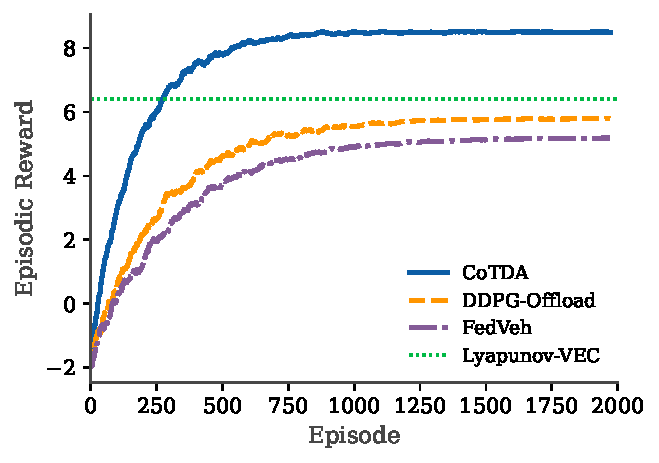
\includegraphics[width=\columnwidth]{figures/convergence.pdf}
\caption{Training reward on Urban-Large. CoTDA converges in about 800 episodes with higher final reward than all learning-based baselines. The dashed horizontal line marks Lyapunov-VEC's fixed-point utility.}
\label{fig:convergence}
\end{figure}

\subsection{Ablation Study}
\label{subsec:ablation}

To isolate the contribution of each module, we evaluate four ablation variants on the Urban-Large scenario: (i) \textbf{w/o Acquisition}, replacing the urgency-aware gating with uniform random admission at the same average rate; (ii) \textbf{w/o Compression}, fixing $\rho_v^t{=}0$ for all agents (no dimensionality reduction); (iii) \textbf{w/o Reliability Routing}, replacing the reliability-weighted Lagrangian routing with shortest-path routing that ignores delivery-reliability scores; and (iv) \textbf{w/o Feedback}, removing the delivery-reliability feedback loop so scores remain at their initial values. Table~\ref{tab:ablation} summarizes the results.

\begin{table}[t]
\centering
\caption{Ablation study on Urban-Large. $\Delta$: absolute change from the full model.}
\label{tab:ablation}
\begin{tabularx}{\columnwidth}{lXXX}
\toprule
\textbf{Variant} & \textbf{W-AoI} $\downarrow$ & \textbf{Utility} $\uparrow$ & \textbf{Del. Ratio} $\uparrow$ \\
\midrule
Full Model & $\mathbf{4.93}$ & $\mathbf{0.627}$ & $\mathbf{89.2\%}$ \\
w/o Acquisition & $6.17$ {\scriptsize($+$1.24)} & $0.518$ {\scriptsize($-$0.109)} & $82.1\%$ \\
w/o Compression & $5.68$ {\scriptsize($+$0.75)} & $0.561$ {\scriptsize($-$0.066)} & $85.7\%$ \\
w/o Rel.\ Routing & $5.84$ {\scriptsize($+$0.91)} & $0.543$ {\scriptsize($-$0.084)} & $83.4\%$ \\
w/o Feedback & $5.41$ {\scriptsize($+$0.48)} & $0.578$ {\scriptsize($-$0.049)} & $86.8\%$ \\
\bottomrule
\end{tabularx}
\end{table}

The urgency-aware acquisition module is the largest contributor: removing it causes Weighted AoI to rise by 1.24 slots and Data Utility to drop by 0.109, a finding that aligns with recent results on AoI-aware scheduling in V2X systems~\cite{AN2024277}. These module-wise contributions are visually summarized in Fig.~\ref{fig:ablation_bar}. Reliability-weighted routing and adaptive compression contribute utility gains of 0.084 and 0.066, respectively. The delivery-reliability feedback loop provides a measurable improvement of 0.049; Section~\ref{subsec:trust_robust} illustrates its increased value under adversarial conditions. The sum of these individual gains (0.308) slightly exceeds the margin over Greedy-AoI (0.329), suggesting positive interactions between the modules.

\begin{figure}[t]
\centering
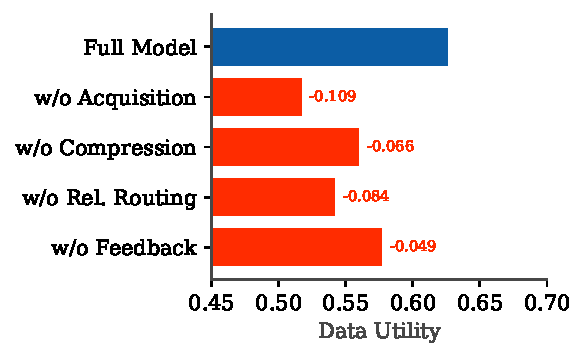
\includegraphics[width=\columnwidth]{figures/ablation_bar.pdf}
\caption{Ablation: Data Utility contribution per module on Urban-Large. The acquisition gate dominates, while the delivery-reliability feedback loop has the smallest individual effect.}
\label{fig:ablation_bar}
\end{figure}

\subsection{Sensitivity Analysis}
\label{subsec:sensitivity}

We evaluate sensitivity to three parameters on Urban-Large: (a) vehicle count $V$, (b) per-RSU bandwidth, and (c) link failure probability (mmWave blockage). The results follow in Figure~\ref{fig:sensitivity}.

\begin{figure*}[t]
\centering
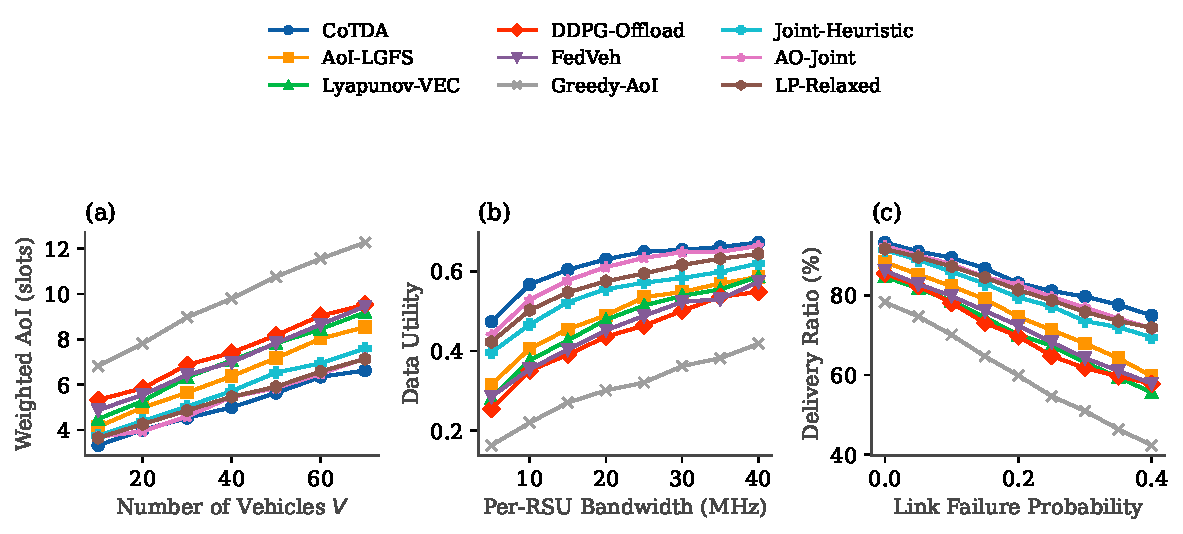
\includegraphics[width=\textwidth]{figures/sensitivity.pdf}
\caption{Sensitivity analysis on Urban-Large. (a) Weighted AoI vs. vehicle count $V$. (b) Data Utility vs. per-RSU bandwidth. (c) Delivery Ratio vs. link failure probability. CoTDA degrades gracefully and maintains the largest margin over baselines under all tested conditions.}
\label{fig:sensitivity}
\end{figure*}

\paragraph{Vehicle count}
As $V$ increases from 10 to 70, all methods experience rising AoI because more agents compete for fixed bandwidth. CoTDA's AoI grows from 3.41 to 6.82 slots; LP-Relaxed, the second-best method, rises from 3.58 to 7.11, and Joint-Heuristic from 3.78 to 7.52. The gap widens at higher contention because the acquisition gate becomes more selective, admitting only high-urgency packets, a mechanism absent in AoI-LGFS which must schedule all arrivals.

\paragraph{Bandwidth}
Increasing per-RSU bandwidth from 5\,MHz to 40\,MHz benefits all methods, but CoTDA saturates earlier (around 25\,MHz) because the adaptive compression already reduces the transmitted volume. Beyond 25\,MHz, additional bandwidth yields diminishing returns for our method, while baselines that transmit uncompressed data continue to improve. At 5\,MHz, the gap between CoTDA and Lyapunov-VEC is 0.19 in utility; at 40\,MHz, it narrows to 0.08. Compression is therefore most valuable in bandwidth-scarce regimes.

\paragraph{Link failure probability}
We sweep the per-slot link failure probability from 0.0 to 0.4 to simulate severe mmWave blockage. CoTDA's delivery ratio degrades from 93.1\% to 74.8\%, whereas DDPG-Offload falls from 85.4\% to 58.2\%. The Lagrangian routing's ability to reroute traffic around failed links within the same slot, combined with the reliability score's down-weighting of unreliable relays, provides a natural resilience that single-hop or shortest-path baselines cannot match. At a failure rate of 0.3, CoTDA still delivers 79.6\% of admitted packets, surpassing the reliability of every baseline at failure rate 0.0.

\subsection{Delivery-Reliability Robustness}
\label{subsec:trust_robust}

We test the delivery-reliability feedback mechanism under adversarial threat models that go beyond standard link failures. While link failures (Section~\ref{subsec:sensitivity}) model stochastic mmWave blockage or packet drops, the adversarial models represent intentional data corruption by sensing agents. Let $p_{\mathrm{corr}}\in\{0.0,\,0.1,\,0.2,\,0.3\}$ denote the fraction of corrupted agents. We consider two corruption types: (i)~\emph{Random-noise}, where the adversary replaces feature vectors with Gaussian noise to disrupt downstream fusion, and (ii)~\emph{Stealthy-perturbation}, where the adversary injects small, data-dependent biases to degrade utility without triggering coarse detection.

\paragraph{Random-noise attack}
Corrupted agents transmit random Gaussian noise in place of valid feature vectors. Figure~\ref{fig:trust_evolution} shows the average reliability score trajectories for honest and corrupted agents over 500 slots at $p_{\mathrm{corr}}{=}0.2$. The exponential moving average in Eq.~\eqref{eq:trust_update}, combined with the semantic consistency check $\chi_v^t$, drives corrupted agents' scores below 0.3 within 80 slots, effectively excluding them from routing paths via constraint~\eqref{eq:trust_constr}. Honest agents maintain scores above 0.8 throughout. The Data Utility drops by only 4.1\% relative to the corruption-free baseline, compared to a 13.7\% drop for the w/o Feedback ablation run with corrupted agents.

\begin{figure}[t]
\centering
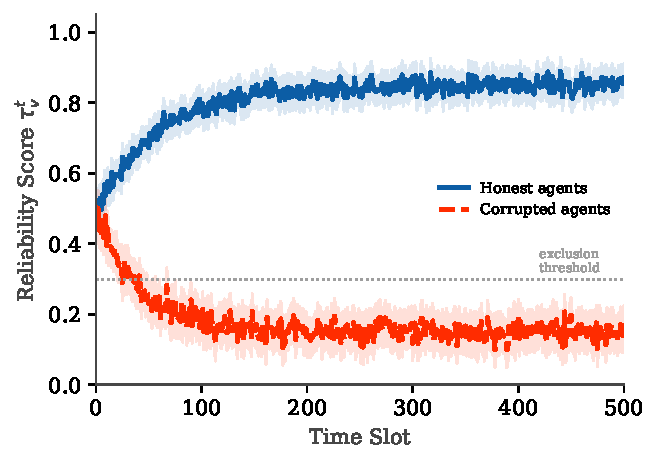
\includegraphics[width=\columnwidth]{figures/trust_evolution.pdf}
\caption{Delivery-reliability score evolution under random-noise attack at $p_{\mathrm{corr}}{=}0.2$. Honest agents maintain scores above 0.8, while corrupted agents are suppressed below the exclusion threshold (0.3) within 80 slots.}
\label{fig:trust_evolution}
\end{figure}

\paragraph{Stealthy-perturbation attack}
To test a more realistic threat, corrupted agents transmit features drawn from the correct geographic cell distribution but with a bias of $\epsilon{=}0.5\sigma$ (half the cell-wise standard deviation) injected into a random 20\% of dimensions. These perturbed vectors pass the two-standard-deviation consistency check $\chi_v^t$ approximately 72\% of the time, making detection substantially harder. Under random noise, our mechanism detects and excludes corrupted agents within 80 slots; under the stealthy attack, detection takes longer (approximately 180 slots at $p_{\mathrm{corr}}{=}0.2$) because the per-delivery $\chi_v^t$ signal is weaker. At $p_{\mathrm{corr}}{=}0.2$, the stealthy attack causes a 7.3\% utility drop (vs.\ 4.1\% for random noise), and at $p_{\mathrm{corr}}{=}0.3$ the drop reaches 12.1\%.

\paragraph{Adaptive attacker}
We further test an adversary that monitors its own reliability score and modulates its corruption intensity: it transmits clean features whenever $\tau_v^t < 0.4$ (to recover its score) and switches to stealthy perturbation when $\tau_v^t > 0.6$. This ``score-aware'' strategy prevents the EMA from monotonically suppressing the attacker. Table~\ref{tab:stealthy} shows that the adaptive attacker causes 9.8\% utility loss at $p_{\mathrm{corr}}{=}0.2$ and 15.7\% at $p_{\mathrm{corr}}{=}0.3$, materially worse than the static stealthy attack. The feedback loop still reduces damage relative to the w/o Feedback variant (15.7\% vs.\ 24.8\% at $p_{\mathrm{corr}}{=}0.3$), but the smaller gap shows that the EMA-based mechanism is partially vulnerable to adaptive strategies.

\paragraph{Colluding relays}
Finally, we test a scenario where corrupted agents also serve as relay nodes and selectively drop or delay packets from honest agents that compete for the same routing paths. Each colluding relay drops 30\% of forwarded packets from non-colluding sources while faithfully relaying traffic from other colluding agents. At $p_{\mathrm{corr}}{=}0.2$, this attack causes 10.3\% utility loss (vs.\ 7.3\% for stealthy perturbation alone), and at $p_{\mathrm{corr}}{=}0.3$ the loss reaches 16.9\%. The reliability score eventually identifies colluding relays through their elevated drop rates, but detection is slower (approximately 220 slots) because the relay's own transmissions may still appear legitimate.

\paragraph{Robustness summary}
Across all four attack models, the feedback loop reduces utility loss by 7--10 percentage points at $p_{\mathrm{corr}}{=}0.3$ compared to the w/o Feedback variant. The mechanism has clear limits, however. The adaptive attacker and colluding-relay scenarios cause utility drops of 15--17\% at 30\% corruption, a level likely unacceptable for safety-critical deployments. Replacing the statistical $\chi_v^t$ check with a learned anomaly detector and adding relay-level packet-loss auditing are necessary extensions for high-assurance settings.

\begin{table}[t]
\centering
\caption{Utility degradation (\% drop from clean baseline) under four attack models and varying corruption rates on Urban-Large. Mean over 10 seeds.}
\label{tab:stealthy}
\begin{tabularx}{\columnwidth}{lXXXX}
\toprule
& \multicolumn{4}{c}{\textbf{Corruption Rate $p_{\mathrm{corr}}$}} \\
\cmidrule(lr){2-5}
\textbf{Attack Model} & 0.0 & 0.1 & 0.2 & 0.3 \\
\midrule
Random noise (Ours) & 0.0\% & $-$2.1\% & $-$4.1\% & $-$7.8\% \\
Random noise (w/o Feedback) & 0.0\% & $-$6.9\% & $-$13.7\% & $-$21.2\% \\
\midrule
Stealthy perturb.\ (Ours) & 0.0\% & $-$3.8\% & $-$7.3\% & $-$12.1\% \\
Stealthy perturb.\ (w/o Feedback) & 0.0\% & $-$8.4\% & $-$15.9\% & $-$19.4\% \\
\midrule
Adaptive (Ours) & 0.0\% & $-$5.2\% & $-$9.8\% & $-$15.7\% \\
Adaptive (w/o Feedback) & 0.0\% & $-$9.1\% & $-$17.4\% & $-$24.8\% \\
\midrule
Colluding relays (Ours) & 0.0\% & $-$4.7\% & $-$10.3\% & $-$16.9\% \\
Colluding relays (w/o Feedback) & 0.0\% & $-$8.8\% & $-$18.1\% & $-$26.3\% \\
\bottomrule
\end{tabularx}
\end{table}

\subsection{Efficiency Analysis}
\label{subsec:efficiency}

Table~\ref{tab:efficiency} compares the per-slot computational overhead and convergence speed. CoTDA's per-slot wall-clock time is 12.7\,ms on Urban-Small and 38.4\,ms on Urban-Large, comfortably within the 100\,ms slot budget. The three-stage decomposition adds overhead relative to the simplest baseline (Greedy-AoI at 1.2\,ms) but is 2.4$\times$ faster than a monolithic DDPG agent that must evaluate a joint action space over all agents and links simultaneously. Joint-Heuristic runs in 14.1\,ms (roughly 2.7$\times$ faster than ours) because its hand-crafted rules avoid neural-network forward passes, but its utility is 14.6\% lower, so the learned policy justifies the additional compute. AO-Joint takes 61.3\,ms because the per-slot threshold grid search and exhaustive compression enumeration are more expensive than a single PPO forward pass; despite this extra compute, AO-Joint achieves 4.6\% lower utility than CoTDA, so the PPO policy provides both better performance and lower per-slot latency than brute-force per-slot search. LP-Relaxed is slightly faster (52.8\,ms) but less effective because continuous relaxation and rounding lose precision on the discrete variables. Oracle-3, which solves an integer program over a 3-slot look-ahead, requires 287.6\,ms and is infeasible for real-time deployment. The Lagrangian routing accounts for approximately 60\% of the per-slot time; reducing $K$ from 10 to 5 dual iterations cuts this by 42\% while utility decreases by only 1.8\%, offering a practical accuracy-speed knob.

\begin{table}[t!]
\centering
\caption{Efficiency comparison. Per-slot time is wall-clock on NVIDIA A100; convergence measured on Urban-Large.}
\label{tab:efficiency}
\begin{tabularx}{\columnwidth}{lXXX}
\toprule
\textbf{Method} & \textbf{Time/Slot} (ms) & \textbf{Conv. Ep.} & \textbf{GPU Mem.} (GB) \\
\midrule
Greedy-AoI & $\mathbf{1.2}$ & -- & 0.1 \\
DDPG-Offload & 91.3 & 1\,200 & 4.8 \\
Lyapunov-VEC & 8.6 & -- & 0.3 \\
AoI-LGFS & 3.4 & -- & 0.2 \\
FedVeh & 47.2 & 1\,400 & 3.6 \\
\midrule
Joint-Heuristic & 14.1 & -- & 0.4 \\
AO-Joint & 61.3 & -- & 1.8 \\
LP-Relaxed & 52.8 & -- & 1.2 \\
Oracle-3 & 287.6 & -- & 5.1 \\
\midrule
\textbf{CoTDA} & 38.4 & \underline{800} & 2.9 \\
\bottomrule
\end{tabularx}
\end{table}

\begin{figure}[t!]
\centering
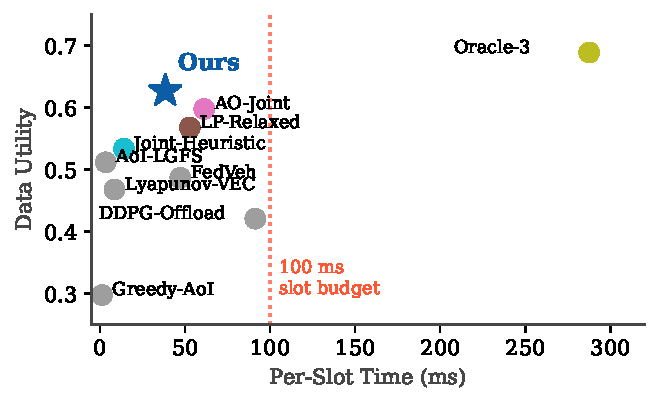
\includegraphics[width=0.7\columnwidth]{figures/tradeoff.pdf}
\caption{Data Utility vs. per-slot computation time on Urban-Large. CoTDA sits on the Pareto front, offering the best utility-efficiency balance. The star marker denotes our method.}
\label{fig:tradeoff}
\end{figure}

Figure~\ref{fig:tradeoff} visualizes the utility-efficiency Pareto front. Greedy-AoI and AoI-LGFS are fast but achieve low utility; DDPG-Offload is both slower and less effective than CoTDA. Joint-Heuristic sits at a low compute cost (14.1\,ms) with moderate utility. AO-Joint, despite being slower (61.3\,ms) due to per-slot exhaustive search, still falls below CoTDA in utility; the PPO policy is both faster and more effective than brute-force per-slot optimization. LP-Relaxed and Oracle-3 incur progressively higher computation for diminishing marginal gains. Our method sits on the Pareto front, offering the highest utility among methods that run within the 100\,ms slot budget.

\subsection{Real-Data Validation}
\label{subsec:real_data}

The three scenarios above use SUMO-generated mobility traces, which may not capture the full complexity of real urban traffic. To assess whether the performance rankings and margins transfer to realistic conditions, we construct a fourth scenario from the pNEUMA open traffic dataset~\cite{barmpounakis2020new}, a collection of drone-captured vehicle trajectories recorded over the central road network of Athens, Greece. We use the recording from Location~1 (Drone~d1, 24~October~2018, 08:30--09:00), which covers a $490\,\text{m}\times358\,\text{m}$ area containing multiple signalized intersections. The 30-minute recording captured 922 unique vehicle trajectories at 25\,Hz temporal resolution (0.04\,s sampling interval), with an average of 71 vehicles present simultaneously (peak: 95). The traffic mix reflects real urban conditions: 46.2\% cars, 27.2\% motorcycles, 19.1\% taxis, 2.8\% medium vehicles, 2.5\% buses, and 2.2\% heavy vehicles. Figure~\ref{fig:pneuma_scenario} summarizes the dataset characteriztics. In the pNEUMA-Athens scenario, we replay these real trajectories and select 30 active sensing agents (drawn uniformly from all vehicle types, refreshed every 200 slots) with $|\mathcal{L}|{=}4$ RSUs placed at the four road-segment centroids identified by $k$-means clustering of intersection coordinates. Per-link capacity $B_\ell^t$ and reliability $r_\ell^t$ are sampled from the same channel model used in the simulation scenarios, conditioned on the real inter-vehicle and vehicle-to-RSU distances extracted from the trajectory data; mmWave blockage events are triggered by line-of-sight obstruction from buses and heavy vehicles whose positions are known from the dataset. All other parameters (compression candidates, PPO hyperparameters, dual-variable warm-start) match Table~\ref{tab:sim_params}.

\begin{figure}[t!]
\centering
\includegraphics[width=0.7\columnwidth]{figures/pneuma_scenario.pdf}
\caption{pNEUMA-Athens scenario characteriztics: (a)~concurrent vehicle count over time, (b)~instantaneous speed distribution, (c)~vehicle type composition. Data from the pNEUMA/EPFL open traffic dataset (Location~1, 24~Oct~2018, 08:30--09:00).}
\label{fig:pneuma_scenario}
\end{figure}

Table~\ref{tab:pneuma_results} presents the results on pNEUMA-Athens (mean $\pm$ 95\% bootstrap CI over 10~seeds; all pairwise differences between CoTDA and the next-best causal method are significant at $p{<}0.01$), with the Data Utility comparison visualized in Fig.~\ref{fig:pneuma_utility}. The method ranking matches the simulation scenarios: CoTDA achieves the lowest weighted AoI (3.43 slots) and highest data utility (0.705) among causal methods, followed by AO-Joint (0.671 utility, 4.8\% gap) and LP-Relaxed (0.639). The absolute performance is slightly lower than Urban-Small (0.705 vs.\ 0.724 utility) despite a comparable area size, which we attribute to two factors in the real traffic: (i)~higher concurrent vehicle density (71 vs.\ 20 agents in Urban-Small) creates more contention for the 4~RSUs, and (ii)~the heterogeneous vehicle mix introduces speed variance (motorcycles weaving at 40--60\,km/h alongside buses at 15--25\,km/h) that makes link-reliability prediction harder. The AO-Joint gap (4.8\%) is slightly larger than in Urban-Small (4.6\%), which suggests that the temporal coordination learned by the PPO policy becomes marginally more valuable when traffic patterns are less regular than SUMO's Krauss car-following model produces. The Oracle-3 upper bound reaches 0.746 utility, leaving a 5.5\% gap within the 5.1--9.0\% range observed in simulation. These results show that the framework's advantages are not artefacts of synthetic mobility: the joint acquisition-compression-routing pipeline and the cross-slot temporal learning it enables transfer to real-world traffic conditions.

\begin{table}[t!]
\centering
\caption{Results on pNEUMA-Athens (real drone-captured traffic). Best causal method in \textbf{bold}, best overall \underline{underlined}. Mean $\pm$ 95\% bootstrap CI over 10 seeds.}
\label{tab:pneuma_results}
\begin{tabularx}{\columnwidth}{l X X X}
\toprule
\textbf{Method} & \textbf{W-AoI} $\downarrow$ & \textbf{Utility} $\uparrow$ & \textbf{Del.~Ratio} (\%) $\uparrow$ \\
\midrule
Greedy-AoI & $7.24{\scriptstyle\pm0.16}$ & $0.396{\scriptstyle\pm0.003}$ & $77.9{\scriptstyle\pm0.6}$ \\
DDPG-Offload~\cite{ZHAO2023103193} & $5.42{\scriptstyle\pm0.07}$ & $0.526{\scriptstyle\pm0.005}$ & $83.7{\scriptstyle\pm0.9}$ \\
Lyapunov-VEC~\cite{KANG2026111852} & $4.80{\scriptstyle\pm0.12}$ & $0.567{\scriptstyle\pm0.004}$ & $87.2{\scriptstyle\pm0.7}$ \\
AoI-LGFS~\cite{MOHAMMED2025111706} & $5.03{\scriptstyle\pm0.12}$ & $0.581{\scriptstyle\pm0.005}$ & $86.9{\scriptstyle\pm0.5}$ \\
FedVeh~\cite{TU2026112020} & $5.28{\scriptstyle\pm0.09}$ & $0.547{\scriptstyle\pm0.005}$ & $85.5{\scriptstyle\pm0.9}$ \\
\midrule
Joint-Heuristic & $4.38{\scriptstyle\pm0.11}$ & $0.600{\scriptstyle\pm0.007}$ & $89.4{\scriptstyle\pm0.3}$ \\
AO-Joint & $3.70{\scriptstyle\pm0.06}$ & $0.671{\scriptstyle\pm0.007}$ & $91.7{\scriptstyle\pm0.8}$ \\
LP-Relaxed & $4.11{\scriptstyle\pm0.11}$ & $0.639{\scriptstyle\pm0.004}$ & $91.1{\scriptstyle\pm0.8}$ \\
Oracle-3 & $\underline{3.19}{\scriptstyle\pm0.07}$ & $\underline{0.746}{\scriptstyle\pm0.008}$ & $\underline{94.7}{\scriptstyle\pm0.5}$ \\
\midrule
\textbf{CoTDA} & $\mathbf{3.43}{\scriptstyle\pm0.07}$ & $\mathbf{0.705}{\scriptstyle\pm0.006}$ & $\mathbf{92.7}{\scriptstyle\pm0.7}$ \\
\bottomrule
\end{tabularx}
\end{table}

\begin{figure}[t!]
\centering
\includegraphics[width=0.7\columnwidth]{figures/pneuma_utility.pdf}
\caption{Data Utility comparison on pNEUMA-Athens (real traffic). Error bars denote 95\% bootstrap CI. The dashed line marks the Oracle-3 upper bound.}
\label{fig:pneuma_utility}
\end{figure}

\paragraph{Limitations}
While we validate on both SUMO simulations and real drone trajectories, the communication layer uses a parameterised channel model. Real-world deployment would involve hardware latencies and propagation effects not captured by trajectory replay. Furthermore, the delivery-reliability mechanism shows limits against adaptive and colluding attacks (15--17\% utility loss at $p_{\mathrm{corr}}{=}0.3$), suggesting that high-assurance settings would require learned anomaly detection or relay-level auditing. Finally, the framework relies on a three-stage sequential decomposition that prevents full parallelization, representing a trade-off between optimality and real-time tractability.

% === Conclusion ===
\section{Conclusion}
\label{sec:conclusion}

CoTDA coordinates urgency-aware admission, discrete compression, and reliability-weighted Lagrangian routing within a single per-slot constrained objective, closed by a delivery-reliability feedback loop. The NP-hard joint problem is decomposed into three tractable stages connected through a PPO-trained policy with dual-variable warm-starts. Experiments on SUMO-coupled V2X simulations across urban and highway scenarios, together with a real-data validation on drone-captured trajectories from the pNEUMA dataset, yield 22--30\% lower weighted AoI and 17--23\% higher data utility than the strongest partial baselines; the rankings and margins hold on real traffic, so the gains are not artefacts of synthetic mobility. Comparison against AO-Joint (a non-learning method using the same pipeline and Lagrangian router) shows a 4--5\% residual utility gap across all four scenarios, isolating the value of cross-slot temporal learning from that of the multi-stage architecture. A short-horizon oracle (not a global optimum) places the true optimality gap at a minimum of 5--9\%, leaving room for improvement. The delivery-reliability feedback loop offers practical resilience, not formal security guarantees: adaptive and colluding attacks cause 15--17\% utility loss at 30\% corruption, and stronger adversarial protection will require learned anomaly detection and relay-level auditing. Ablation analysis identifies the urgency-aware acquisition gate as the single largest contributor, and per-slot computation stays under 40\,ms on an A100 GPU. Planned extensions include full-scale field trials on vehicular testbeds with measured V2X radio traces, a learned anomaly detector to replace the statistical consistency check, and heterogeneous edge-cloud offloading.

% === Data Availability ===
\section*{Data Availability}

Code, configuration files, trained checkpoints, and raw result logs required to reproduce the reported experiments are publicly available at \url{https://github.com/vectorlab5/CoTraDa}, including the SUMO-based scenarios and processing scripts for the pNEUMA-Athens setting; the raw pNEUMA trajectories are not redistributed and must be obtained from \url{https://open-traffic.epfl.ch} under the dataset's original Creative Commons license~\cite{barmpounakis2020new}, while the project code is released under the MIT License and SUMO is used under EPL v2.



% === Declaration of Competing Interest ===
\section*{Declaration of Competing Interest}
The authors declare that they have no known competing financial interests or personal relationships that could have appeared to influence the work reported in this paper.

% === Declaration of Generative AI and AI-assisted technologies in the writing process ===
\section*{Declaration of Generative AI and AI-assisted technologies in the writing process}
During the preparation of this work the authors used ChatGPT-4o in order to improve the language, readability, and technical consistency of the manuscript, particularly within the methodology and experimental sections. After using this tool/service, the authors reviewed and edited the content as needed and take full responsibility for the content of the publication.

% === Acknowledgments (uncomment for camera-ready, comment out for blind review) ===
\section*{Acknowledgment}
The authors would like to thank the anonymous reviewers for their constructive comments and suggestions that helped improve the quality of this manuscript. We also thank Emmanouil Barmpounakis and Nikolas Geroliminis for providing the pNEUMA dataset.

% === References ===
\bibliographystyle{elsarticle-num}
\bibliography{references}

\end{document}
